\documentclass[authoryear,preprint,12pt]{elsarticle}

% Load necessary packages
\usepackage[margin=1.5cm]{geometry}
\usepackage{natbib}
\usepackage{csquotes}
\usepackage{stmaryrd}
\usepackage{mathtools,amsfonts,amssymb,setspace}
\usepackage{amsmath}
\usepackage{amssymb}
\usepackage{array} 
\usepackage{caption}
\usepackage{subcaption}
\usepackage{ragged2e}
\usepackage{textgreek}
\usepackage{hyperref}
\usepackage{tikz}
\usepackage{tabularx}
\usepackage{adjustbox}
\usepackage{lipsum}
\usepackage{titlesec}

\begin{document}

\title{Operational long-term management of a salt cavern for industry targeted green H2 production}

\author{First Name Last Name}
\ead{youremail@example.com}

\address{Paris-Saclay University}

\begin{abstract}
    An abstract to paste
\end{abstract}

\begin{keyword}
keyword1 \sep keyword2 \sep keyword3
\end{keyword}

\maketitle

\clearpage
\section{Introduction}
\label{Intro}

HELLO HELLO
\subsection{Context}

The utilization of hydrogen stands as a pivotal step towards combating climate change through the decarbonization of industrial processes, transportation and the seamless integration of variable renewable energy sources into the electricity grid \citep{shukla2022climate}.
Presently, there is a significant global upsurge in the demand for hydrogen, highlighting its increasing importance across various sectors \citep{iea_global_2022}. Especially for industry, hydrogen can be converted into ammonia in order to be primarily used for fertilizers. 
\\

As stated beforehand, the future industrial green H2 production plant will be large and probably associated to large salt cavern. The latter means that an optimized operational management, i.e. an Energy Management Systems (EMS), should allow for consequent financial savings. However, this EMS will face the following challenges: 
\begin{itemize}
    \item The horizon of prediction of renewable productions does not exceed few days while the system is equipped with a storage which capacity exceeds weeks of production. This time-scale mismatch leads to the necessity of adding long-term management capabilities to the EMS.
    \item Within the industrial context, the green H2 must be produced respecting constraints such as CO2 content \citep{green_hydrogen_organisation_green_2023} or rate of production to match the low flexibility of downstream processes such as Haber-Bosch ammonia production reactor \citep{shamiri_modeling_2021}.
\end{itemize}
In the present work, an EMS that accounts for long-term management and industrial constraints is developed in order to evaluate the financial savings obtained on a large-scale plant.


\subsection{State-of-the-art}
The existing literature offers a rich array of methodologies for constructing EMS \citep{weitzel_energy_2018}. As summarized by \cite{alabi_strategic_2023}, the two advanced EMS methodologies that can cope with the dynamic variations of smart energy systems are Model Predictive Control (MPC) and Reinforcement Learning (RL). The latter approaches are illustrated by \cite{stoffel_evaluation_2023}, in the context of building energy management systems, who compared traditional reactive expert rules to model-free RL, MPC based on white-box, gray-box and black-box modeling and approximate MPC. While RL seems promising, there are still scientific challenges to overcome such as its lake of explicability, the effective management of specific constraints and the necessary consequent offline training on precise simulators. Those are probably the reasons why the studies that have probed the domain of EMS tailored specifically to hydrogen production in industrial settings are based on MPC.
\\
Noteworthy among these, \cite{klyapovskiy_optimal_2021} showcased the considerable potential of EMS in increasing the economic performance of industrial facilities reliant on hydrogen. Their approach involved the utilization of hydrogen and electricity, partially sourced from local renewables, emphasizing the pivotal role of EMS in optimizing such intricate energy systems, all executed within the framework of a Mixed-Integer Linear Programming (MILP) model. Expanding on this, their approach assesses energy management across four representative days, providing a planning horizon with a renewable production forecast of 24 hours. Such an approach however lacks the management of long term phenomena.
\\
Regarding EMS strategies including long term management but not in the field of hydrogen production, \cite{cuisinier_new_2022,cuisinier_impact_2023} presented a rolling horizon approach based on a MILP model that combines the short term, evaluated hourly, and the long term, evaluated at an arbitrarily longer interval.
The sole decision variable for the long term becomes the variation in the State of Energy (SOE) of the long-term storage, a thermal pit storage associated to district heating in their case. This variable is employed by Cost Functions (CF), which represent the operational cost of the system for a given time interval and for a variation of storage SOE. These CF are precalculated based on numerous MILP models over Representative Periods (RP) of the long term horizon.
\\

Based on the analysis of the state-of-the-art, none of the papers examined cope with industrial constraints such as maximal CO2 content of the produced H2 or minimal H2 rate of production. The most recent and advanced approaches for EMS tailored specifically to hydrogen production in industrial settings are based on hierarchical approaches, that may have difficulties to cope with such constraints. In the field of district heating, the methodological continuous approach of \cite{cuisinier_new_2022} is promising in order to both cope with the long term management of the salt cavern and these industrial constraints.


\section{System investigated and methods}
\subsection{Modeling approach} \label{Models}

The platform is modeled using a MILP formulation. The nomenclature of parameters and decision variables are described in \autoref{tab:system_parameters_and_DV}.
It uses the indice $sys$ for each type of system, with the set of indices for each type of system being described in \autoref{tab:system_description}.
The MILP modeling for the renewable production, grid, converters, compressors and storage is rather common and thus described in \ref{app:model}. As detailed in \ref{app:model}, the grid, converters, compressors and storage sets of equations are respectively denoted \textit{F}, \textit{C}, \textit{K} and \textit{S}.

\begin{table*}
    \centering
    \tiny
    \caption{Parameters and decision variables}
    \begin{tabular}{|p{3.5cm}p{6.5cm}p{5cm}|}
    \hline
    \multicolumn{3}{|c|}{\textbf{(L) Electrolyser}} \\[0.3cm]
    $L^{(k,max/min)}$                   & Max/Min power of the $k^{th}$ electrolyser                                        & $[MW]$ \\
    $L^{(k,AuxBase)}$                   & Base electricity consumption of the $k^{th}$ electrolyser                         & $[MW]$ \\
    $L^{(k,AuxMarg)}$                   & Marginal electricity consumption rate of the $k^{th}$ electrolyser                &  \\
    $L_i^{(k,elec)}$                    & electricity $i^{th}$ operating point of the $k^{th}$ electrolyser                 & $[MW]$ \\
    $L_i^{(k,H_2)}$                     & $H_2$ flow $i^{th}$ operating point of the $k^{th}$ electrolyser                  & $[tH_2/h]$ \\[0.3cm]
    $\textbf{L}_\textbf{t}^{\textbf{(k,elec)}}$           & Electricity consumption of the $k^{th}$ electrolyser at $t$ for $H_2$             & $[MW]$ \\
    $\textbf{L}_\textbf{t}^{\textbf{(k,H$_2$)}}$            & $H_2$ flow production of the $k^{th}$ electrolyser at $t$                         & $[tH_2/h]$ \\
    $\textbf{L}_\textbf{t}^{\textbf{(k,total)}}$          & Total electricity consumption of the $k^{th}$ electrolyser at $t$                 & $[MW]$ \\
    $\textbf{l}_\textbf{t}^{\textbf{(k,state)}}$          & State of the $k^{th}$ electrolyser at $t$ : 1 if turnd on else 0                  & $[MW]$ \\[0.3cm]
    \multicolumn{3}{|c|}{\textbf{Global parameters}} \\[0.3cm]
    $M^{(CO_2)}$                    & Maximum hourly $CO_2$ intensity of $H_2$ sold                                         & $[tCO_2/tH_2]$ \\
    $m^{(H_2)}$                     & Minimum hourly $H_2$ sold quantity                                                    & $[tH_2/h]$ \\
    $\Delta$                        & Duration of rolling constraints                                                       & $[h]$ \\
    $\delta_t$                      & Duration of instant $t$                                                               & $[h]$ \\
    $N_{ely}$                       & Number of electrolysers modules                                                       & \\
    \hline     
    \end{tabular}
    \label{tab:system_parameters_and_DV}
\end{table*}

\clearpage
\appendix

\section{MILP models} \label{app:model}
The present Appendix describes the MILP modeling for the renewable production, grid, converters, compressors and storage.
\subsection{Renewable production} \label{Renewable_production}

PV and wind production are modeled with capacity factor time series considered as inputs for the optimization problem. Thus, no decision variables are related to renewable production.

\subsection{Grid Flow} \label{Grid_Flow} \label{eq:F}
Local electricity grid can consume (related to \textit{ElecCons}) or inject (related to \textit{ElecInj}) electricity from/to the global electricity grid. The local $H_2$ grid can sell $H_2$ (related to \textit{$H_2$sold}). If the platform does not satisfy production or $CO_2$ constraints (see Section \ref{specific_constraints}), it can "buy" expensive external green $H_2$ (related to \textit{$H_2$pen}). \textit{$H_2$pen} can be interpreted as a penalty to prevent unfeasabilty during the platform operation. Equations (\ref{eq:F1}) and (\ref{eq:F2}) set hourly cost and $CO_2$ emissions for each flow, system and instant. Equation (\ref{eq:F3}) sets flow constraints related to infrastructures limitation.

\begin{equation} \tag{F.1} \label{eq:F1}
    \textbf{F}_\textbf{t}^{\textbf{(sys,cost)}} = F^{(sys,sens)} \cdot F_t^{(sys,prices)} \cdot \textbf{F}_\textbf{t}^{\textbf{(sys,flow)}}
\end{equation}
\begin{equation} \tag{F.2} \label{eq:F2}
    \textbf{F}_t^{(sys,CO2)} = F^{(sys,CO_2)} \cdot \textbf{F}_\textbf{t}^{\textbf{(sys,flow)}}
\end{equation}
\begin{equation} \tag{F.3} \label{eq:F3}
    F^{(sys,min)} \leq \textbf{F}_\textbf{t}^{\textbf{(sys,flow)}} \leq F^{(sys,max)}
\end{equation}


\section{MILP tolerance} \label{app:MILP}
In this Appendix, the impact of the modeling of the electrolysers with SOS2 variables is evaluated. The objective is to check that the operating points of the electrolysers on the obtained results do not deviate from the operating curve of \autoref{fig:ely_operating_range}. The gap between operating point given by the EMS and operating curve is calculated with Equation (\ref{eq:L2}). \autoref{fig:ely_gap} provides a visual representation of the gap, demonstrating that only a few operating points are significantly outside the allowed range. 
\begin{equation*}
     \text{Gap}_t = \textbf{L}_\textbf{t}^{\textbf{(k,elec)}} \cdot \alpha_i^{(k)} - \textbf{l}_\textbf{t}^{\textbf{(k,state)}} \cdot \beta_i^{(k)} - \textbf{L}_\textbf{t}^{\textbf{(k,H$_2$)}}
\end{equation*}

\begin{figure}
    \centering
    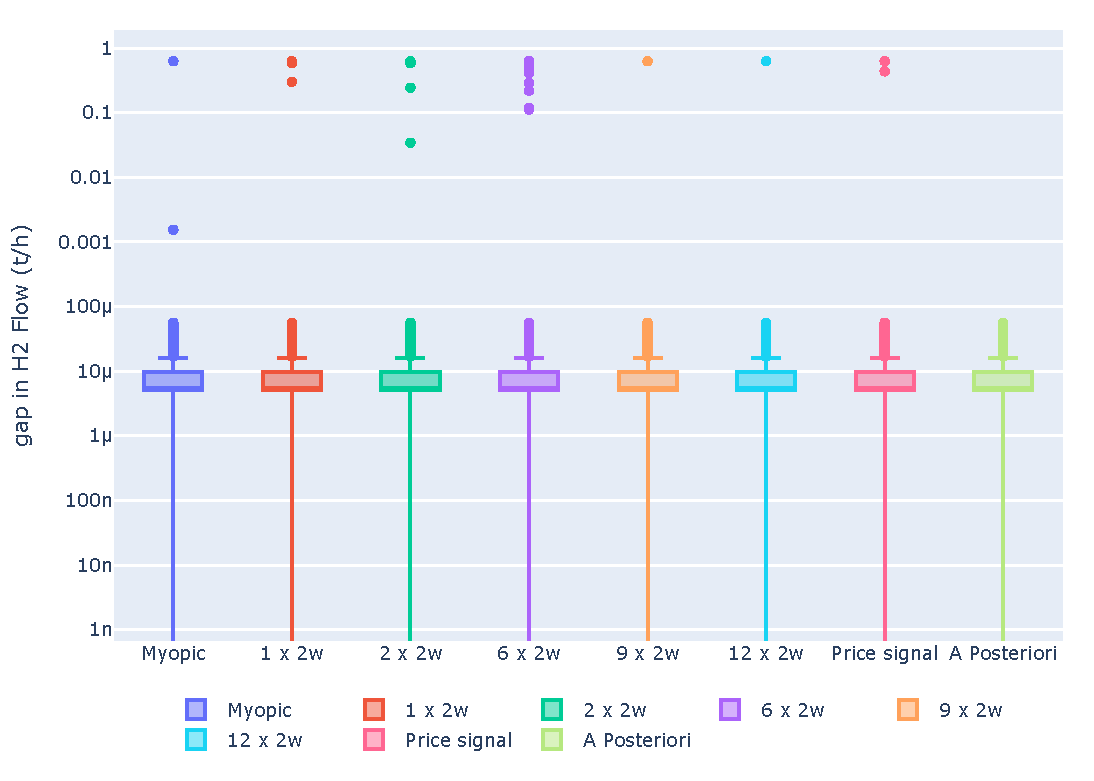
\includegraphics[width=10cm]{02_Appendix/MILP_tolerance_boxplot.pdf}\\
    \caption{Absolute gap between operation range of electrolyser and operating point of the EMS}
    \label{fig:ely_gap}
\end{figure} 

\bibliographystyle{elsarticle-num-names}
\bibliography{ref}

\end{document}
